% !TeX spellcheck = it_IT
\documentclass{llncs}
%%%%%%%%%%%%%%%%%%%%%%%%%%%%%%%%%%%%%%%%%%%%%%%%%%%%%%%%%%%
%% package sillabazione italiana e uso lettere accentate
\usepackage[latin1]{inputenc}
\usepackage[english]{babel}
\usepackage[T1]{fontenc}
%%%%%%%%%%%%%%%%%%%%%%%%%%%%%%%%%%%%%%%%%%%%%%%%%%%%%%%%%%%%%

\usepackage{url}
\usepackage{xspace}
\usepackage{amsmath}
\usepackage{pdfpages}


\makeatletter
%%%%%%%%%%%%%%%%%%%%%%%%%%%%%% User specified LaTeX commands.
\usepackage{manifest}
\usepackage{listings}
\usepackage{textcomp}
\makeatother

\usepackage{tikz}
\usetikzlibrary{arrows,automata}

\newcommand{\java}{\textsf{Java}}
\newcommand{\contact}{\emph{Contact}}
\newcommand{\corecl}{\texttt{corecl}}
\newcommand{\medcl}{\texttt{medcl}}
\newcommand{\msgcl}{\texttt{msgcl}}
\newcommand{\android}{\texttt{Android}}
\newcommand{\dsl}{\texttt{DSL}}
\newcommand{\jazz}{\texttt{Jazz}}
\newcommand{\rtc}{\texttt{RTC}}
\newcommand{\ide}{\texttt{Contact-ide}}
\newcommand{\xtext}{\texttt{XText}}
\newcommand{\xpand}{\texttt{Xpand}}
\newcommand{\xtend}{\texttt{Xtend}}
\newcommand{\pojo}{\texttt{POJO}}
\newcommand{\junit}{\texttt{JUnit}}

\newcommand{\action}[1]{\texttt{#1}\xspace}
\newcommand{\code}[1]{{\small{\texttt{#1}}}\xspace}
\newcommand{\codescript}[1]{{\scriptsize{\texttt{#1}}}\xspace}

% Cross-referencing
\newcommand{\labelsec}[1]{\label{sec:#1}}
\newcommand{\xs}[1]{\sectionname~\ref{sec:#1}}
\newcommand{\xsp}[1]{\sectionname~\ref{sec:#1} \onpagename~\pageref{sec:#1}}
\newcommand{\labelssec}[1]{\label{ssec:#1}}
\newcommand{\xss}[1]{\subsectionname~\ref{ssec:#1}}
\newcommand{\xssp}[1]{\subsectionname~\ref{ssec:#1} \onpagename~\pageref{ssec:#1}}
\newcommand{\labelsssec}[1]{\label{sssec:#1}}
\newcommand{\xsss}[1]{\subsectionname~\ref{sssec:#1}}
\newcommand{\xsssp}[1]{\subsectionname~\ref{sssec:#1} \onpagename~\pageref{sssec:#1}}
\newcommand{\labelfig}[1]{\label{fig:#1}}
\newcommand{\xf}[1]{\figurename~\ref{fig:#1}}
\newcommand{\xfp}[1]{\figurename~\ref{fig:#1} \onpagename~\pageref{fig:#1}}
\newcommand{\labeltab}[1]{\label{tab:#1}}
\newcommand{\xt}[1]{\tablename~\ref{tab:#1}}
\newcommand{\xtp}[1]{\tablename~\ref{tab:#1} \onpagename~\pageref{tab:#1}}
% Category Names
\newcommand{\sectionname}{Section}
\newcommand{\subsectionname}{Subsection}
\newcommand{\sectionsname}{Sections}
\newcommand{\subsectionsname}{Subsections}
\newcommand{\secname}{\sectionname}
\newcommand{\ssecname}{\subsectionname}
\newcommand{\secsname}{\sectionsname}
\newcommand{\ssecsname}{\subsectionsname}
\newcommand{\onpagename}{on page}

\newcommand{\student}{Gruppo 3 Aimi Niccol\'o, Gallegati Mattia, Murgia Antonio, Zanotti Andrea }
\newcommand{\studentEmail}{niccolo.aimi@studio.unibo.it; mattia.gallegati2@studio.unibo.it; antonio.murgia2@studio.unibo.it; andrea.zanotti9@studio.unibo.it}
\newcommand{\xfaculty}{II Faculty of Engineering}
\newcommand{\xunibo}{Alma Mater Studiorum -- University of Bologna}
\newcommand{\xaddrBO}{viale Risorgimento 2}
\newcommand{\xaddrCE}{via Venezia 52}
\newcommand{\xcityBO}{40136 Bologna, Italy}
\newcommand{\xcityCE}{47023 Cesena, Italy}
\lstset{emph={%  
    QActor, System, Plan, Event, host, port, context, Context, [, ], emit%
    },emphstyle={\color{red}\bfseries\underbar}%
}%
%
% Comments
%
%%% \newcommand{\todo}[1]{\bf{TODO:}\emph{#1}}


\begin{document}

\title{Final Theme System\\
 process report}

%%% \author{\xauthA \and \xauthB}
\author{\student}

\institute{%
%%%  \xunibo\\\xaddrCE, \xcityCE\\\email{\{nameA.studentA, nameB.studentB\}@studio.unibo.it}
  \xunibo\\\xaddrBO, \xcityBO\\\email\ {\studentEmail}
}

\maketitle

%% \begin{abstract}
%% \footnotesize
%%This a Latex template to be used for the reports of Software Engineering.
%%\keywords{Software engineering, managed software development, reports, ....}
%%\end{abstract}

%%% \sloppy

%===========================================================================
\section{Introduction}
\labelsec{intro}
In this document we'll describe and discuss the process that led to the development of a robotic software system. We'll discuss how traditional software/project development techniques can and should merge with the scrum project management system.\\ 
We'll face the limits of traditional analysis approaches and purpose novel ones that better match with new programming paradigms.
%===========================================================================

%===========================================================================
\section{Vision}
\labelsec{Vision}
Here we're collecting some visions that will inspire the development of this project and of software in general:\\
\begin{itemize}
	\item There's no code without project, there's no project without problem analysis and there's no problem without requirements;
	\item There's no code without tests. That means that tests must be developed before the development of the software product;
	\item There's no code without documentation;
	\item The team that develops the tests should be different from the one who will realize the project;
	\item We should use a top down approach during the development phase and bottom-up approach during the implementation phase;
	\item Zooming? Trying to get closer..
		We should look at things initially from a far point of view like a black box and then trying to get closer to the details of the system, white box.
	\item Any sufficiently advanced technology is indistinguishable from magic.
	\item Develop the code in an IOT prospective using the ICT principles.
	\item Create valuable software using less time and resource possible in order to optimize software development process (factorization).
	\item A feature does not exist unless a test validates that it functions.
	\item Software entities should be open for extension but closed for modification.
	\item We should always check the existence of prior projects, trends or patterns regarding the technological domain we are facing. If does exist something we should study it, not only to take advantage of it during the development but also to recognize its limits and to purpose some innovative approach coming from different technological domains;
	\item The development of the project should be technology agnostic;
	\item We should find or create a formal language able to describe the results of the problem analysis. It should be similar to spoken language. This language could take advantage of different programming paradigms (functional, declarative and so on) and different programming models (actor model, message passing model and so on). This language should not be tied to any technology implementation. There should be one or more parsers/compilers for this language that will generate source code for a specific platform. This generated code should be used as the skeleton of the real product.
\end{itemize}
%===========================================================================

%===========================================================================
\section{Goals}
\labelsec{Goals}
The first goal is to develop a robotic software system using the most advanced programming paradigms.\\ 
A secondary goal is to develop and to take advantage of a novel technique of requirements and problem analysis that will lead to a formal representation of the problem and to source code generation.
Finally the main goal is discuss how some change (monotonic extensions) of the requirements impact on a product whose production is based on 'formal' and 'technology independent' artifacts rather than on ad-hoc code.
\labelsec{Goals}
%===========================================================================

%===========================================================================
\section{Requirements}
\labelsec{Requirements}
Design and build a (prototype of a) software system that, with reference to a differential drive robot (called from now on robot):
\begin{itemize}
	\item allows a user to select between a 'learning phase' and a 'autonomous phase'
    during the learning phase, the user can send a sequence of move commands (e.g. forward, backward, left right, stop) to the robot. The robot must not only execute each command but it must also record the whole sequence of commands until the user decides to terminate the learning phase;
    \item after the termination of the learning phase, the user can tell the robot to enter the autonomous phase in a 'direct' or in a 'reverse' mode. During this phase the robot executes in autonomous way the sequence of moves it has learned, by complementing each move (e.g. forward->backward) if the selected mode is reverse;
    \item during the autonomous phase, the robot must be able to execute (as soon as possible) a stop command sent by the user.
\end{itemize}
After the development of this prototype, consider the possibility to enhance the functional capabilities of the robot, by allowing it:
\begin{itemize}
	\item to perceive an obstacle during the autonomous phase and, once the obstacle is detected, to execute some alternative behaviour (in term of moves).
\end{itemize}

%===========================================================================

 
%===========================================================================
\section{Requirement analysis}
\labelsec{ReqAnalysis}
%===========================================================================
\subsection{Use cases}
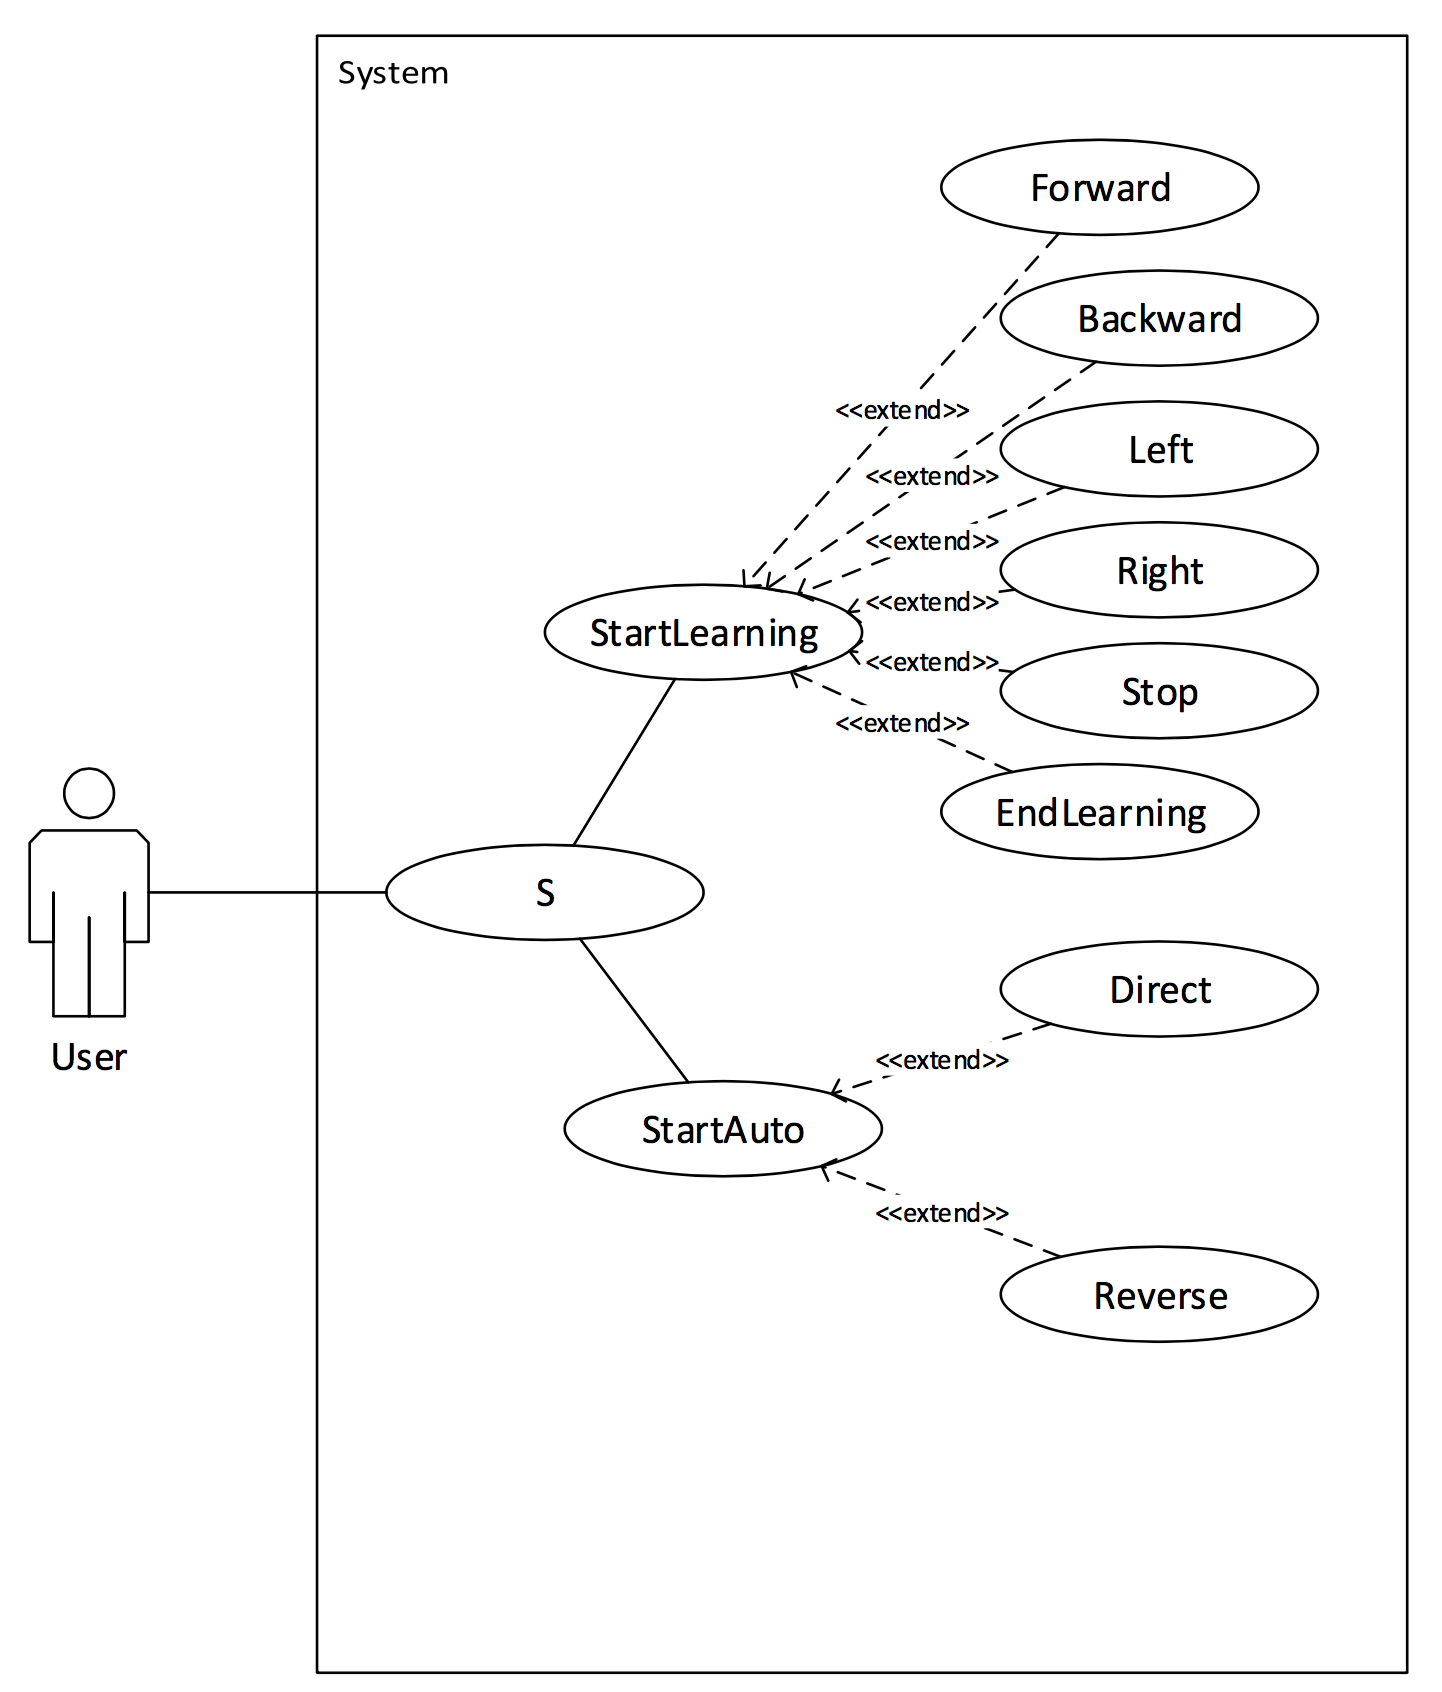
\includegraphics[width=13cm]{img/usecase.png}\\
\labelssec{UseCases}

\subsection{Scenarios}
\labelssec{Scenarios}
\begin{center}
   	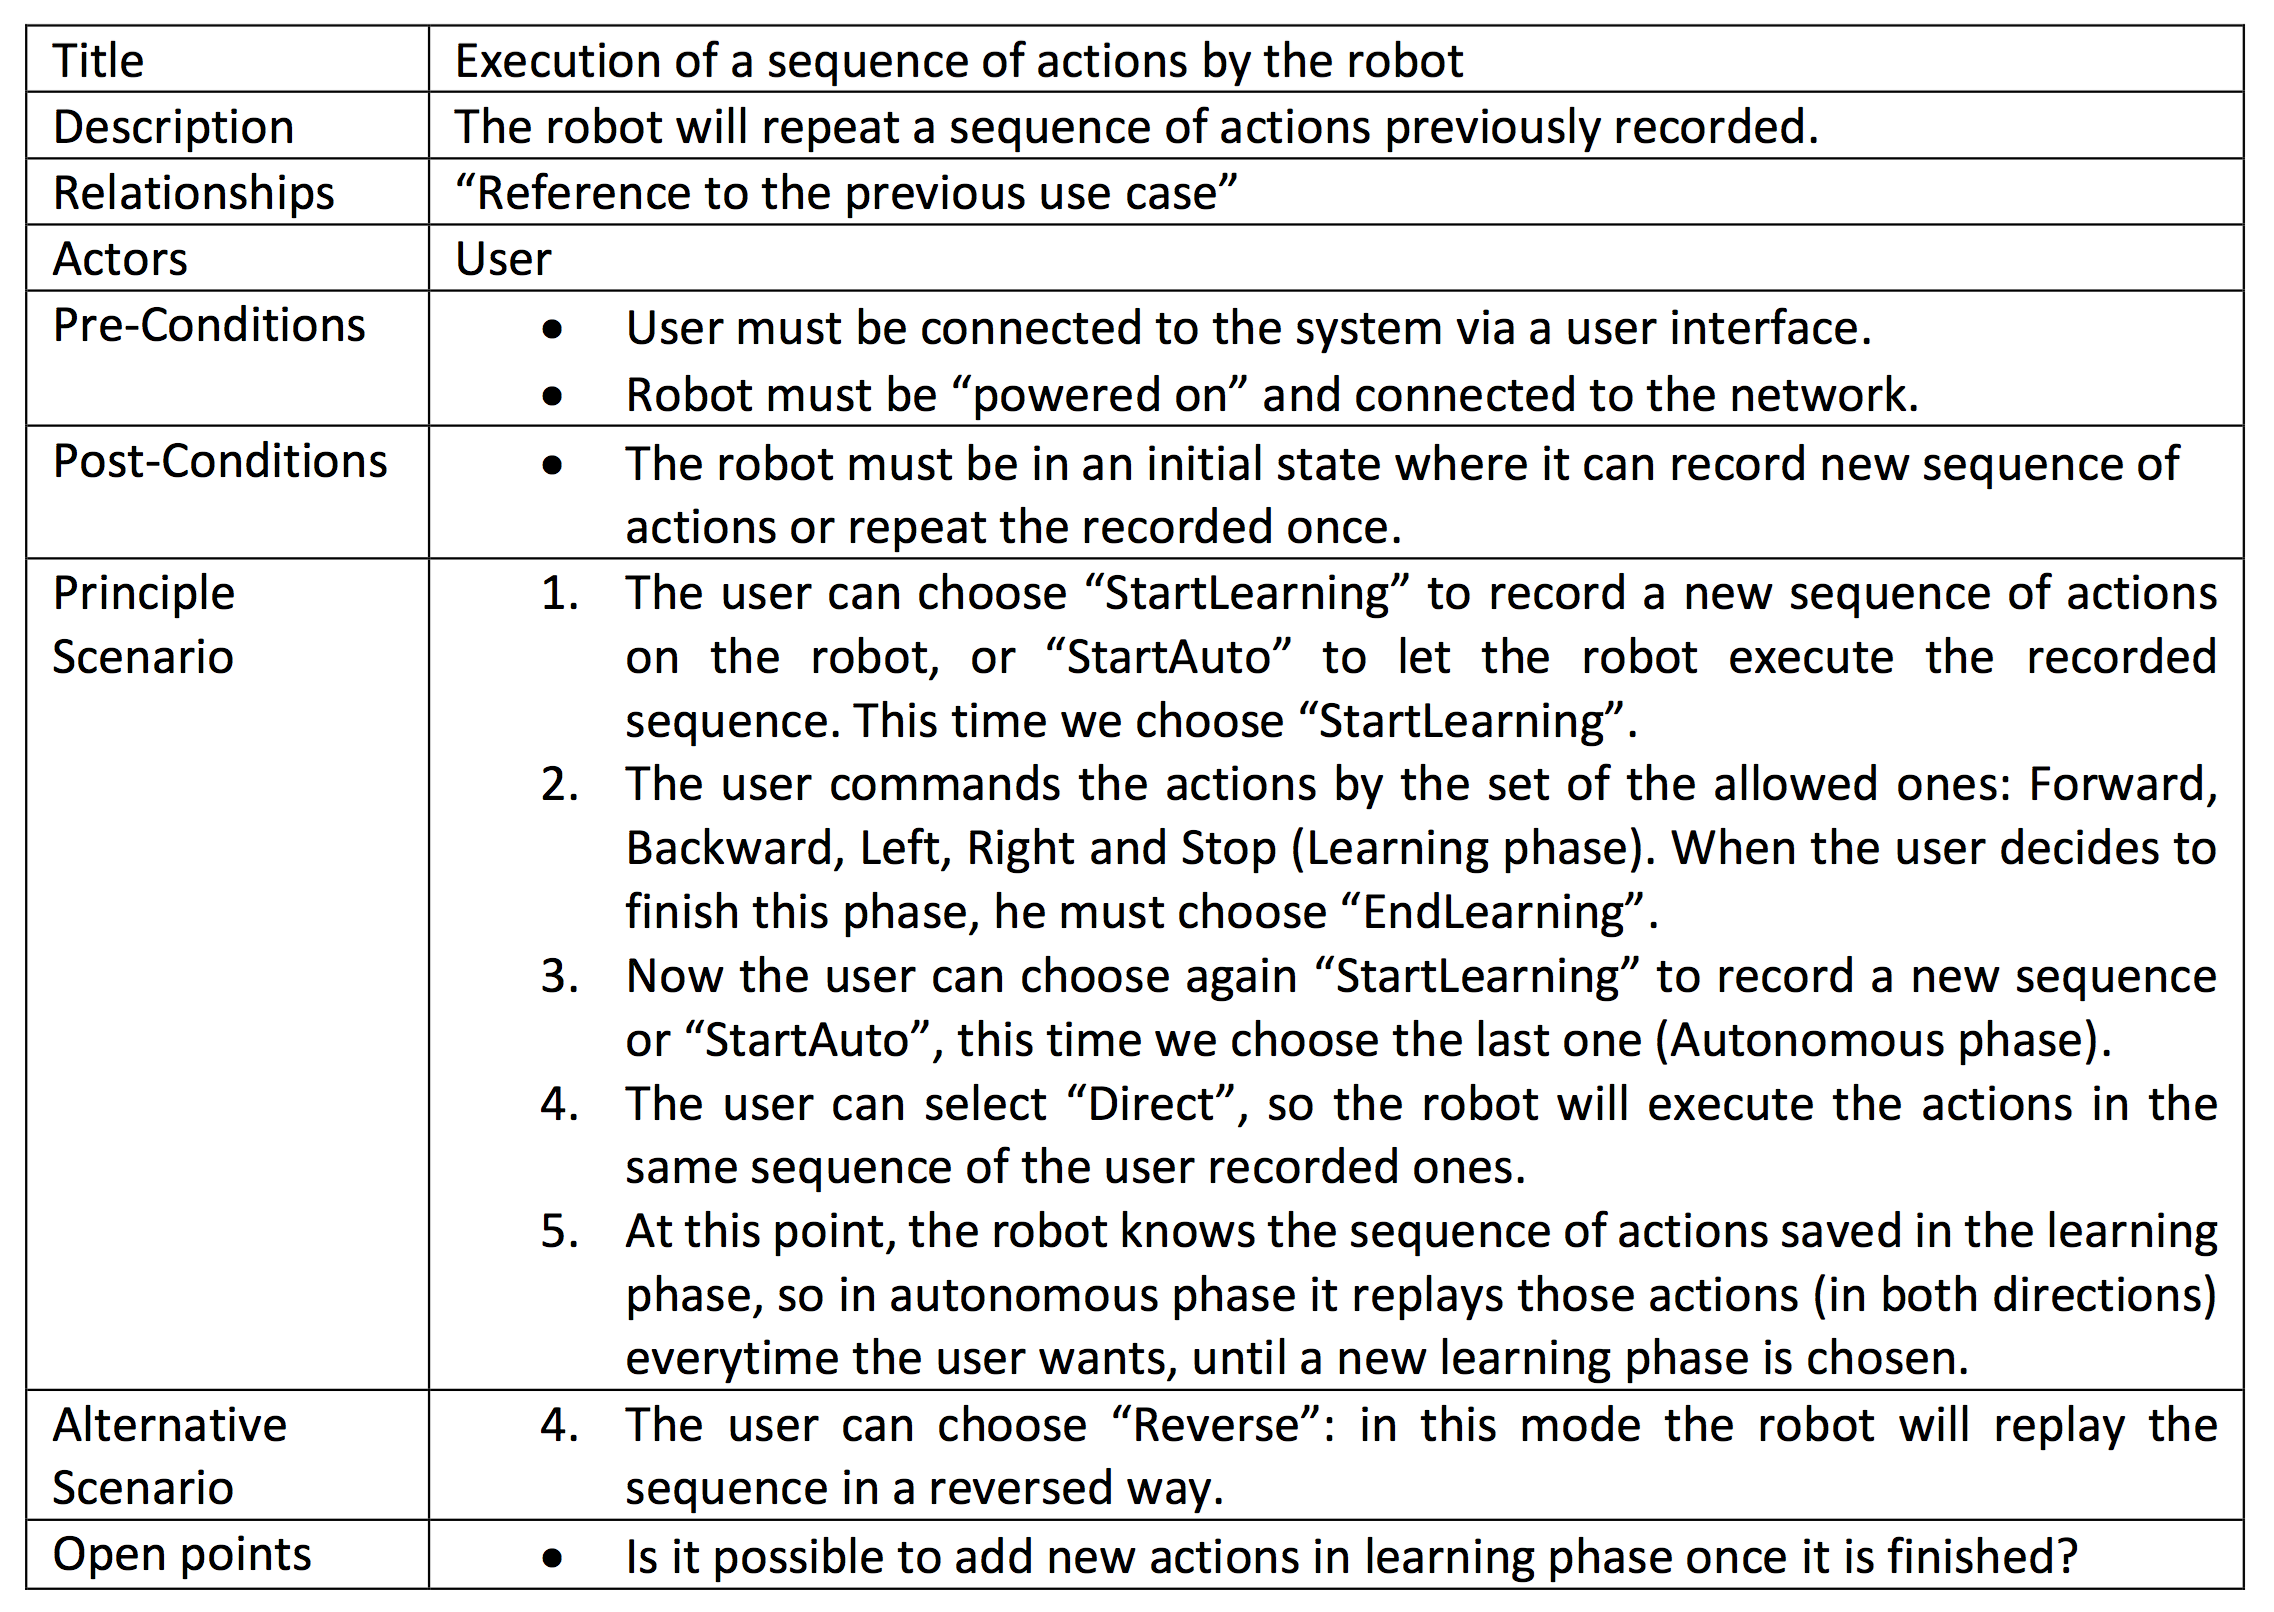
\includegraphics[width=13cm]{img/scenario.png}\\
\end{center}
\subsection{(Domain)model}
\labelssec{(Domain)model}
\paragraph{Structure}
\subsubsection{ROBOT}
We consider the robot as a reactive and atomic entity.
\subsubsection{REMOTE}
We consider the remote as a proactive and atomic entity.
\paragraph{Interaction}
The interaction between the entities of the system is described with this sequence diagram:
\begin{center}
   	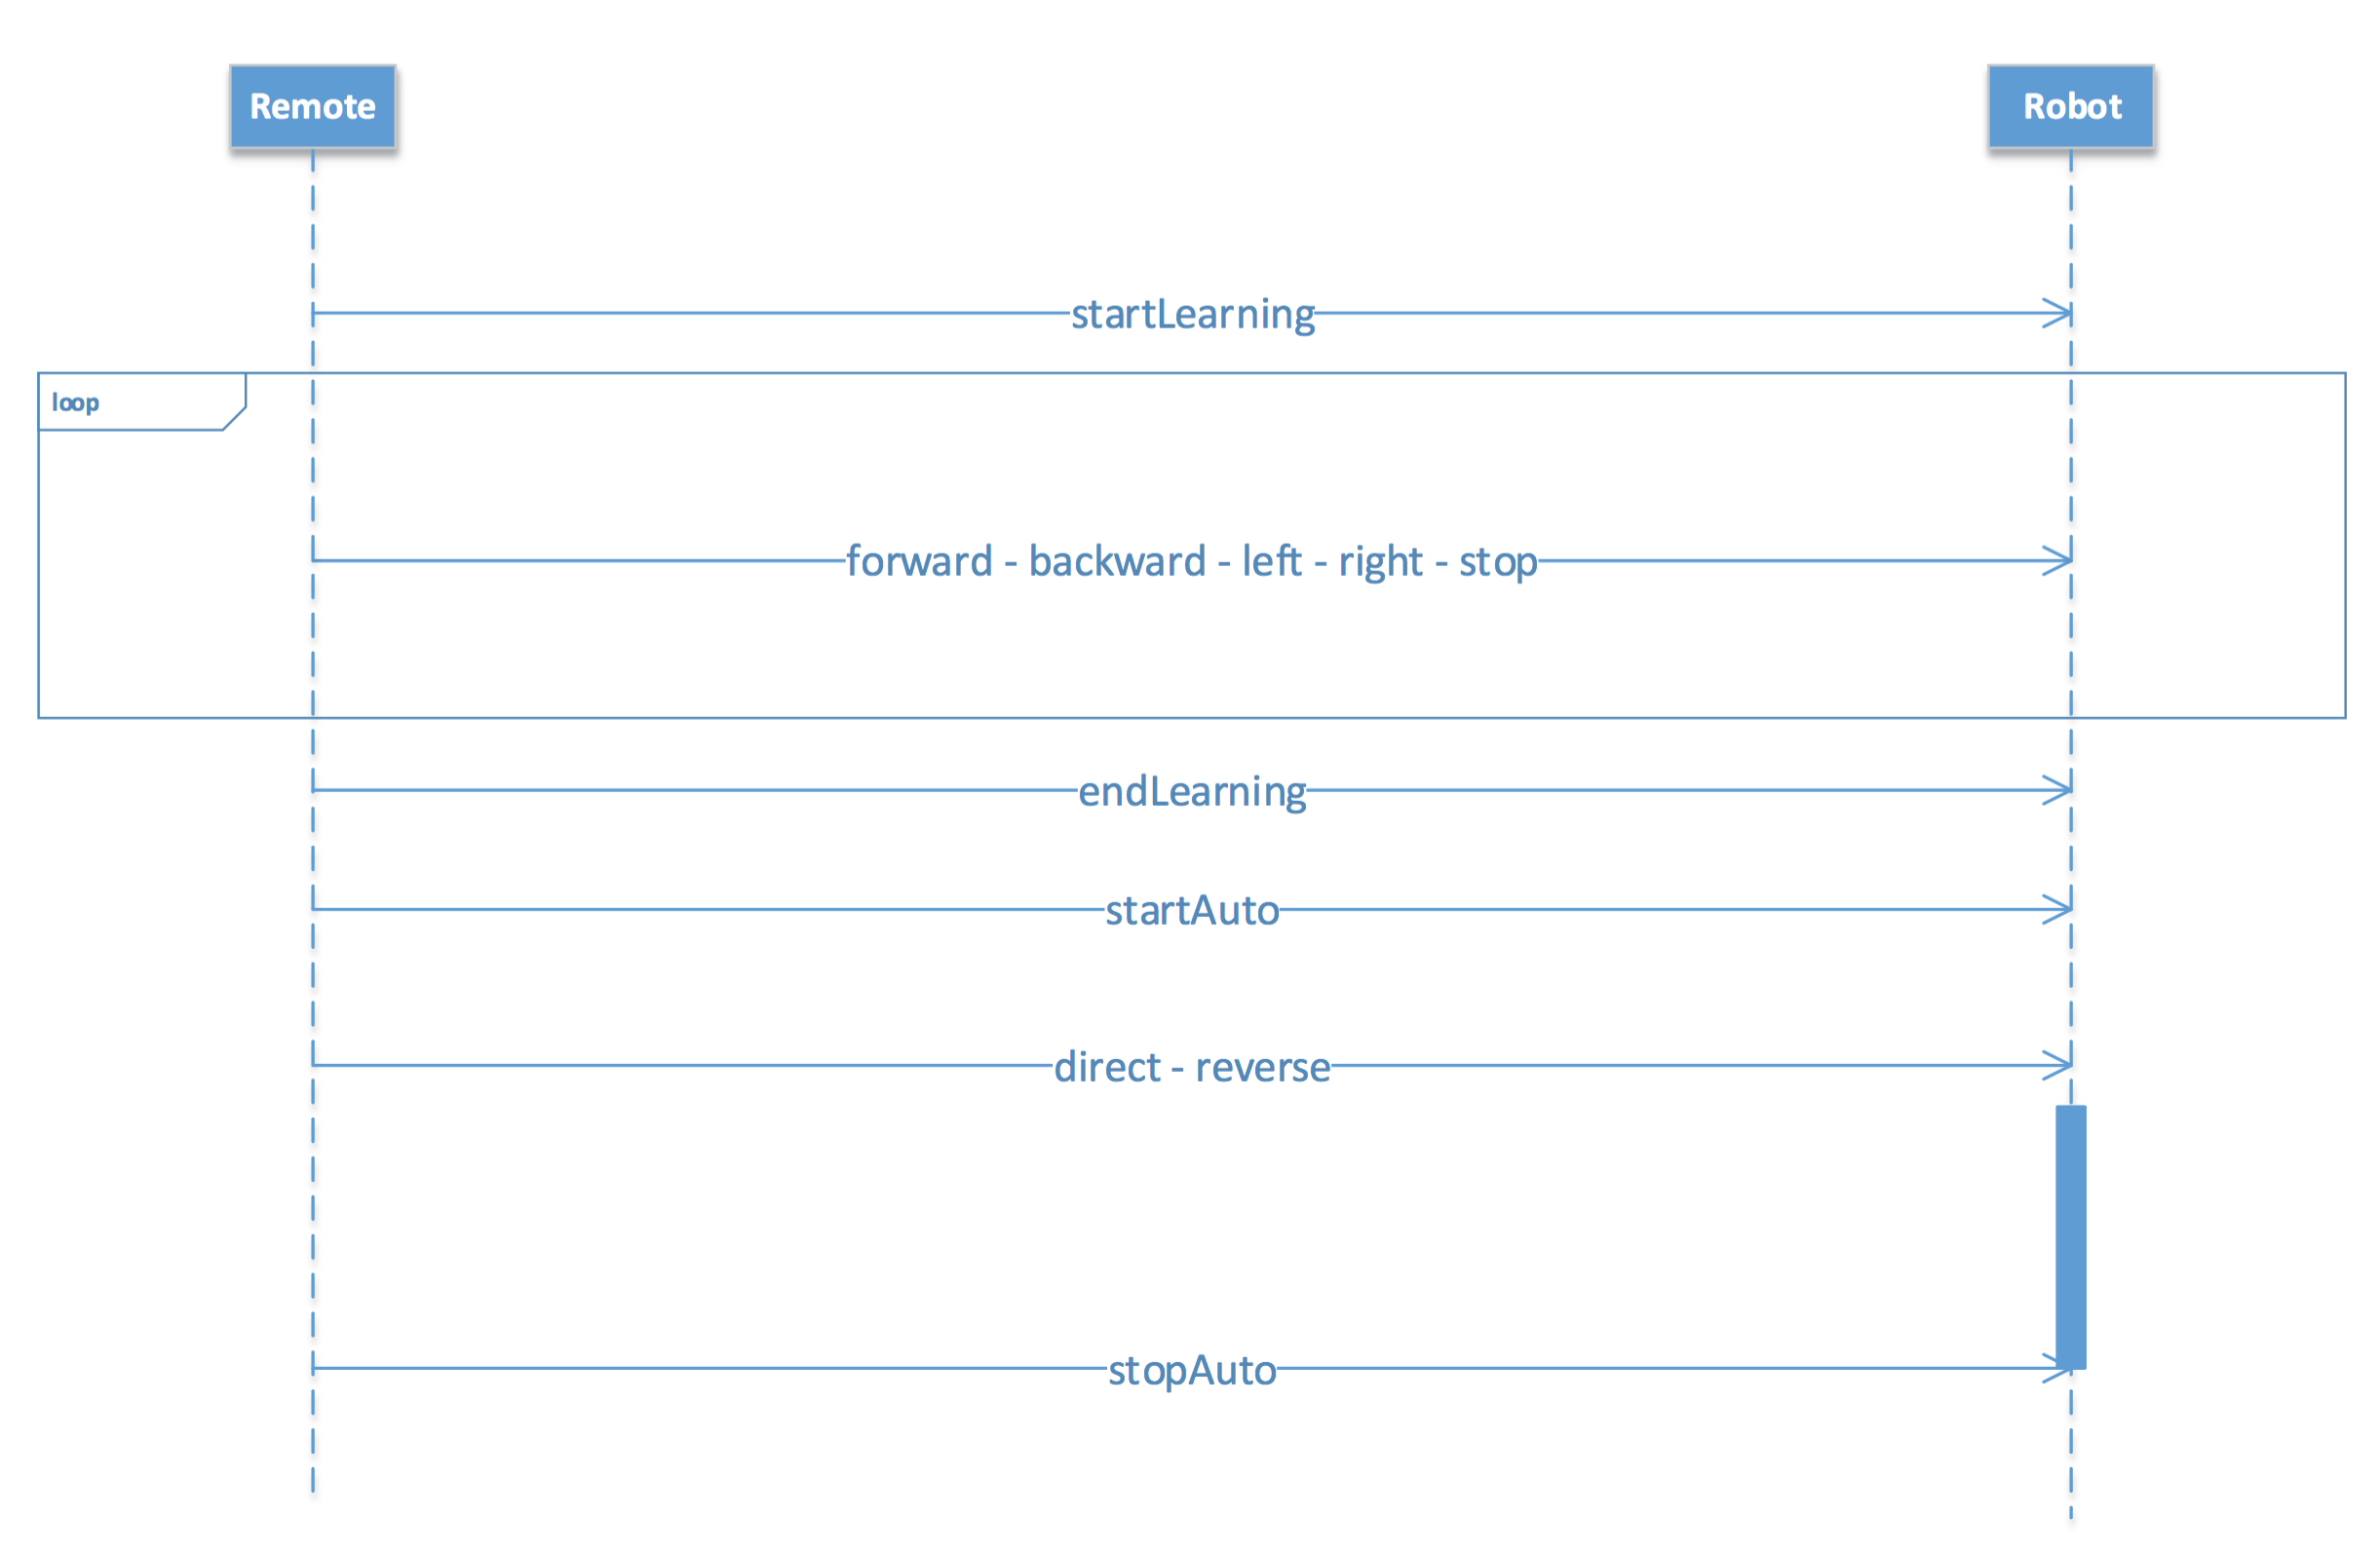
\includegraphics[width=13cm]{img/interaction.png}\\
\end{center}
\paragraph{Behaviour}
\subsubsection{ROBOT}
The behaviour of the robot is described with this FSM:\\
\begin{center}
   	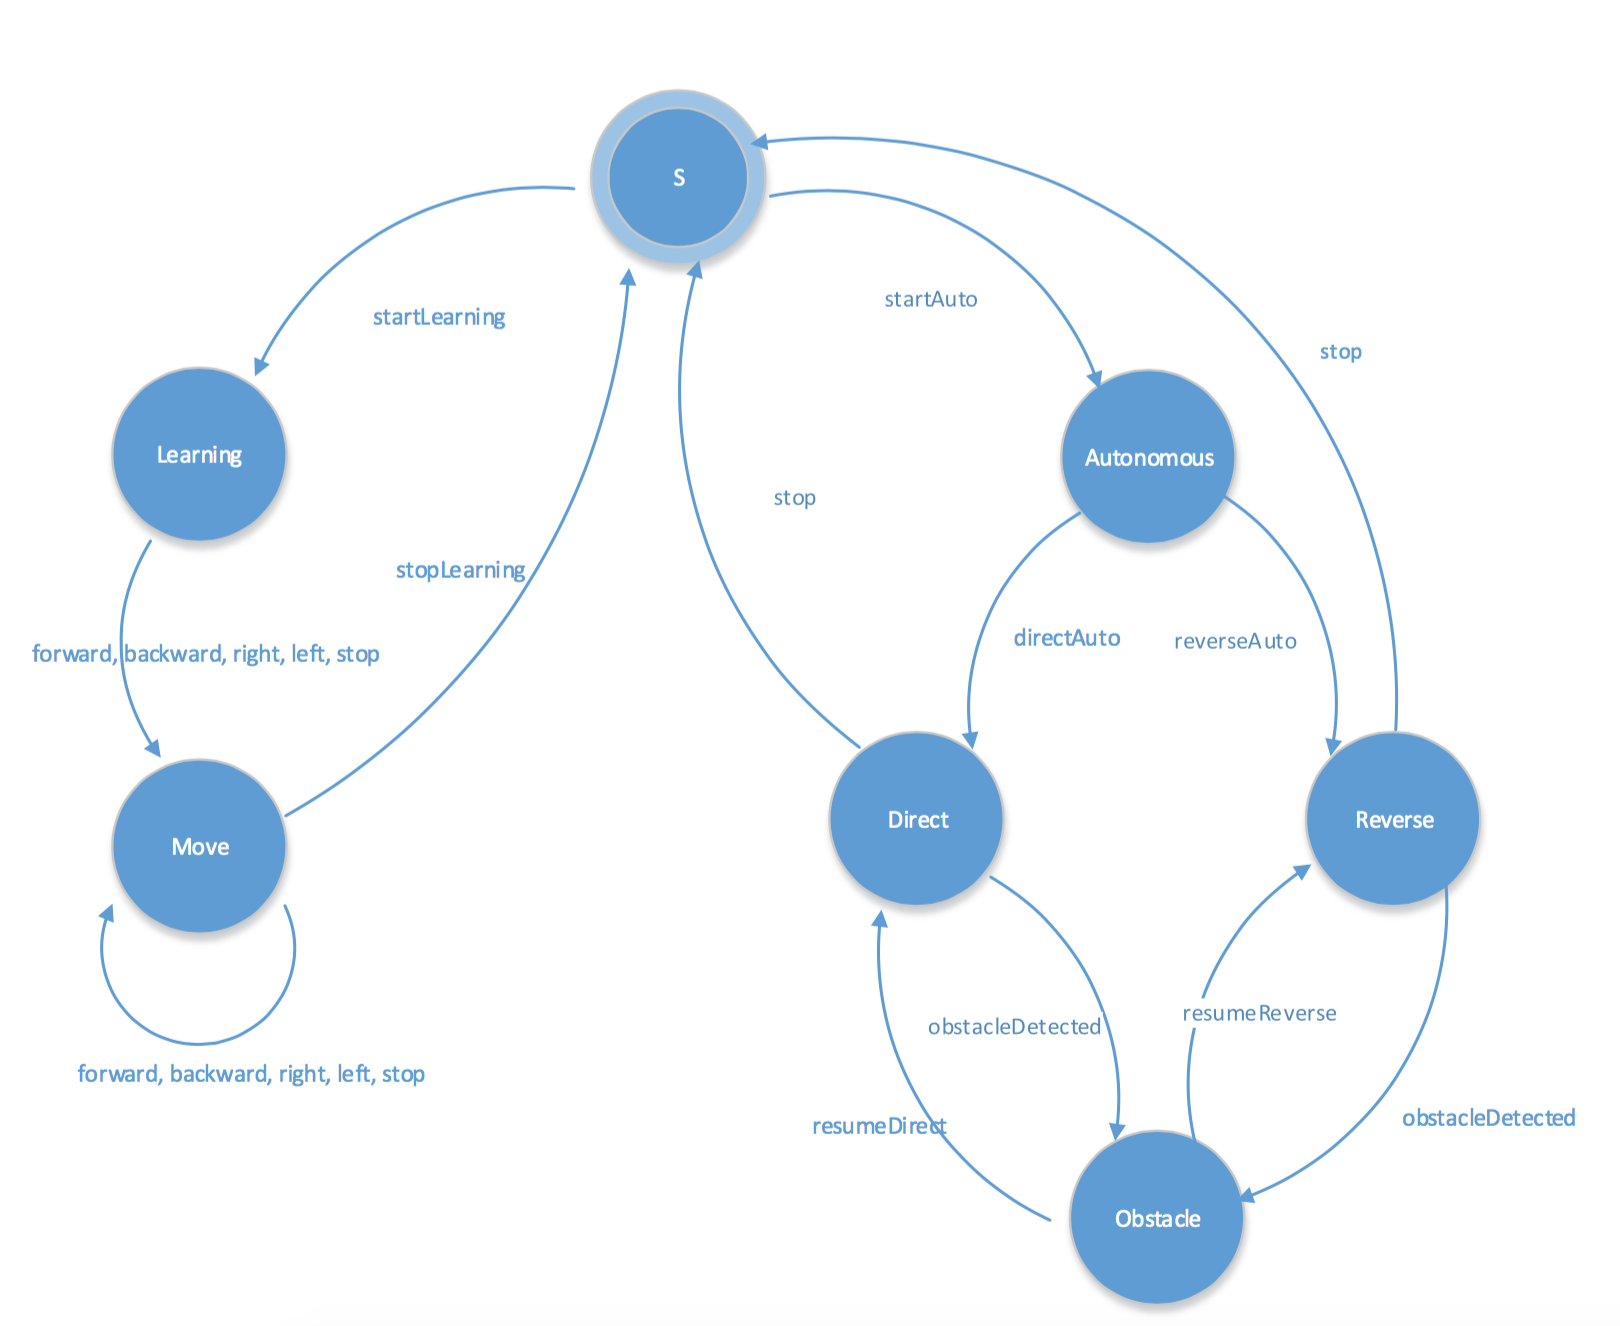
\includegraphics[width=12.5cm]{img/fsmRobot.png}\\
\end{center}
\subsubsection{REMOTE}
The behaviour of the remote is described with this FSM:\\
\begin{center}
   	
\includegraphics[width=2cm]{img/fsmRemoteRequirementAnalysis.png}\\
\end{center}
\subsection{Test plan}
Explaining test plan of a physical system and at this high-level of abstraction in a formal way is still an open point to us. It is not possible to write JUnit tests (that can be reused in the testing process) at this point of the project. Because of the lack of a formal way to define test plans in this chapter we will describe our test plan as natural language:
\begin{itemize}
	\item during the learning phase we check that the robot must react to movement commands;
	\item after the learning phase we check that the recorded actions are the same as the previously executed ones;
	\item we check that the system is responsive only to the meaningful events in every possible state;
	
\end{itemize}
\labelsec{Test plan}
%===========================================================================
\section{Problem analysis}
\labelsec{ProblemAnalysis}
Our technological hypothesis is JAVA and Object Oriented Programming. We will show that we need to develop a new infrastructure because the only features offered by the programming language chosen are not enough.  
To keep our code well developed, scalable, efficient and maintainable, we will use the most known development patterns.
We must define an interaction language, that needs a communication standard. The communication standard will be essential during the Integration Test.
%===========================================================================
\subsection{Abstraction gap}
During the problem analysis we considered Java as our technological hypotesis. We realized that Java's unique communication tool is procedure calls, with OO paradigm it becomes really difficult to implement modular communication where entities are completely independent and loosely coupled. We need a new way to let our components interact.
In agreement with our vision, we understand that the best way to overcome this problem is to develop a new software infrastructure that will map more strictly to our model representation than Java paradigms.
This infrastructure will be used not only in this project, but every future developed process that will have the same needs because, according to our visions, we want to develop reusable code.\\
Our platform must offer some functionalities.
First of all we need a formal definition of a System:\\
a System is one or more active entities that interact to reach some goal or provide some functionalities. A system is composed by one or more Contexts, a Contexts identifies a logical location at deployment time. The System enables the communication between the entities and synchronizes them so Entities must interact using the System only. In this way a System can be concentrated or distributed seamlessly for the application designer.
Defined this general perspective we can introduce two paradigms: 
\begin{itemize}
	\item Message Based Programming
	\item Event Based Programming
\end{itemize}
\subsubsection{Message Based Programming}
	To introduce message based programming we need to define the entities that can exchange messages. We will call these entities QActors in reference to Erlang's Actors.\\ 
	QActors in our platform are not message-driven but message-based. The core difference between message driven and message based is that message driven systems can be only reactive to messages instead of being able to decide when messages and which messages are functional to evaluate. In this way we can model not only reactive entities but also proactive ones. QActors live in a context and they can communicate with other QActors using different communication primitives:
\begin{itemize}
		\item dispatch - an asynchronous message without returning information;
		\item request - a message with returning information, can be executed as synchronous or asynchronous.
\end{itemize}
QActors can receive messages using the receive message primitives:
\begin{itemize}
		\item receiveMessage - extracts the first message from the actor message queue;
		\item receiveTheMessage - extracts the first message that matches a pattern given by the application designer.
\end{itemize}
\subsubsection{Event Based Programming}
	We needed to define the concept of events as pervasive messages that are spread in the system. The message passing paradigm lacks of this feature because all messages are point to point. Events are a form of asynchronous communication that is not point to point. In our system our entities can declare to be interested in an event, when that event will be emitted the entities can react in some way.\\
	When we introduced proactive QActors we realized that we needed the concept of Plan. A Plan is a sequence of actions (you can see actions as programming language instructions), every plan has its own logic and can switch to a different plan. When the execution of a plan reaches its end it can specify if the previous plan must continue its execution or suspend it.
	This abstraction was lacking of the better part of message/event driven programming: reactivity. This gap is filled by Asynchronous Actions.
	Asynchronous Actions are tipically time consuming actions that can be executed in blocking or non-blocking way. When executing an asynchronous action its execution can be interrupted by specified events and the QActor must react executing the associated plan. The logic of plan switching is defined as above.
	QActors are able to execute actions in two ways:
	\begin{itemize}
		\item executing compiled code
		\item interpreting meta code on the fly
	\end{itemize}
Adding the possibility to interpret code on the fly permits to the QActor to enrich its behaviour during runtime.
The just described platform will be realized with Java Programming Language (our technologic assumption) but will be made to be interoperable with other technologies by the extensive use of text-based messages using the standard socket technology.\\
On top of the API offered by the platform we'll realize a DSL using the xtext framework. With the use of such tool we'll generate a declarative language that will provide two main benefits:
\begin{itemize}
	\item a formal and human readable language to describe the problem analysis, entities interactions and system topology;
	\item code generation to be able to customize and execute the artifacts generated by the DSL interpretation.
\end{itemize}
With such tools in mind we can reimagine the traditionals problem analysis techniques and tackle the problems in a formal and more convenient way.
\subsection{Logic architecture}
The logic architecture is shown in the picture below:
\begin{center}
	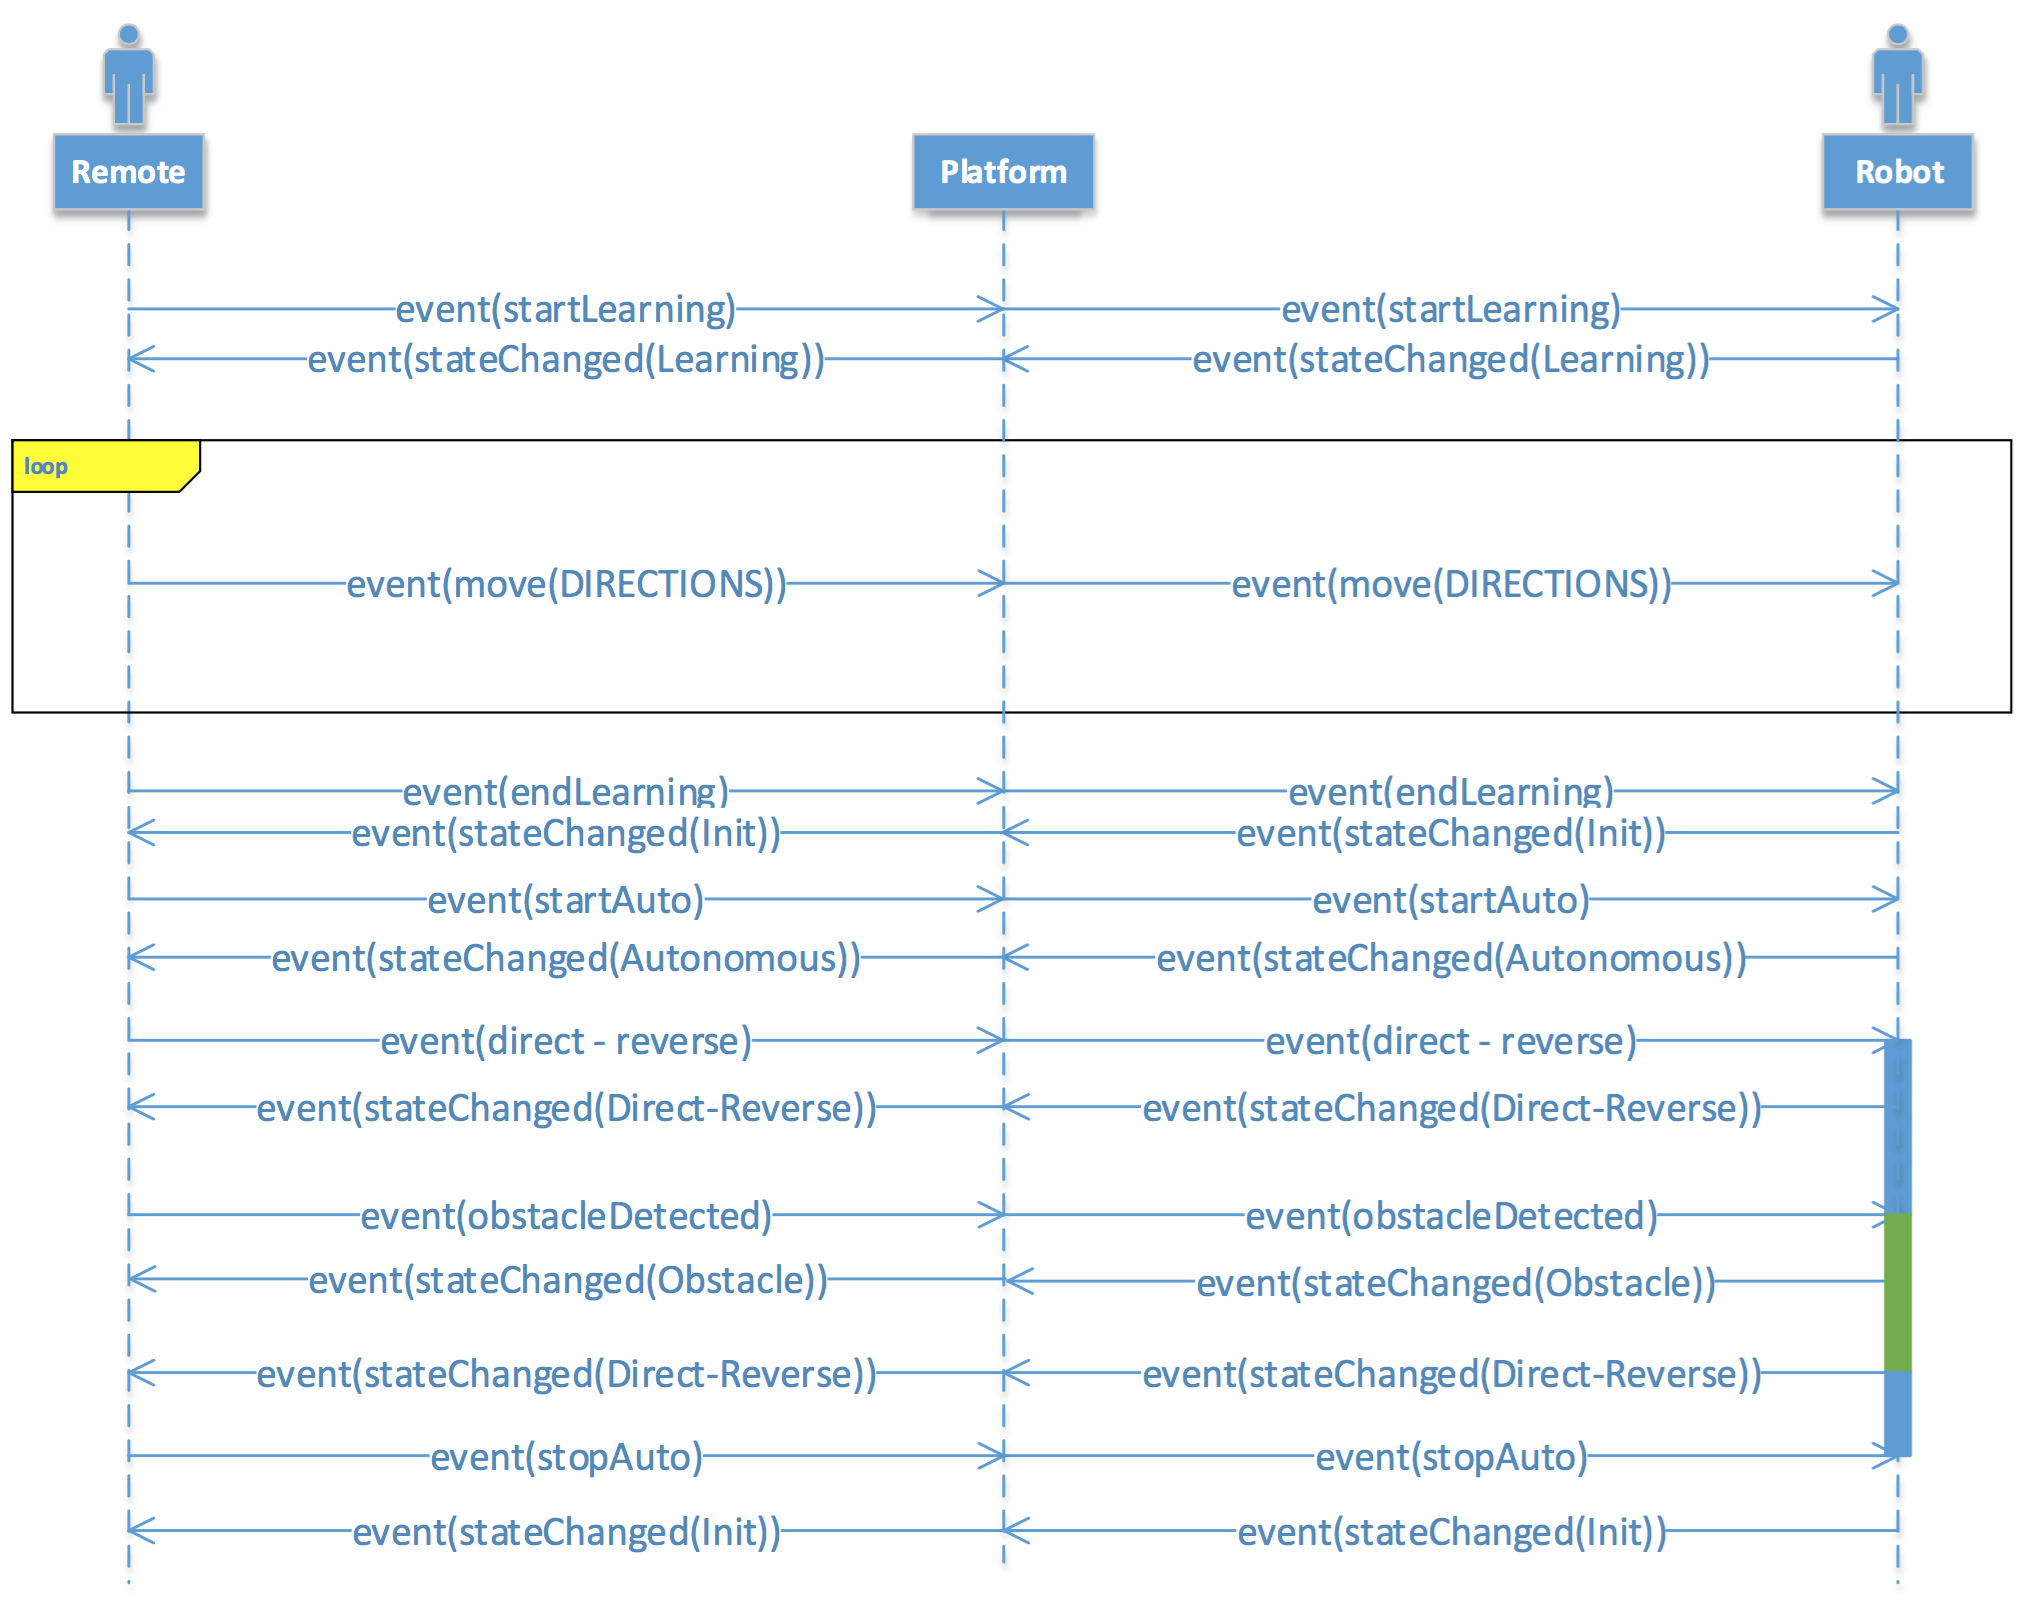
\includegraphics[width=13cm]{img/interaction_problem_analysis.png}
\end{center}
\begin{lstlisting}
System robot

//ChangeStateRobot
Event planChanged:planChanged(CURRENTSTATE)

//LearningPhase
Event moveOrEnd:moveOrEnd(DIRECTION)

//InitialPhase
Event start:start(PHASE)

//Auto Phase
Event mode:mode(AUTOORDIRECT)
Event obstacleDetected:obstacleDetected()
Event stop:stop()

Context  ctxRobot ip [ host="localhost" port=8037 ]
 
Context  ctxRemote ip [ host="localhost" port=8038 ]

QActor qaRobot context ctxRobot {
	Plan init normal 
		println("Robot hello");
		[!! start] getActivationEvent ev
		//delay time(100000) react event startLearning -> learning or event startAutonomous -> autonomous
		
	Plan learning
		println("learning phase");
		[!! moveOrEnd] dummyRobotMove
		// react event move -> learning or event stopLearning -> init
		//[!! moveOrStop]
		//dummyRobotMove react event move -> reactToMove or event stopLearning -> reactToStopLearning;
		//dummyrobotmove � una mossa di movimento e aggiungere la regola in java
		//repeatPlan 1000000
	
	
	Plan autonomous
		println("Autonomous phase")
		//delay time(100000) react event directAutonomous -> direct or event reverseAutonomous -> reverse
		
	Plan obstacle
		println("Obstacle phase");
		delay time(3000);
		println("Obstacle destroyed");
		resumeLastPlan
}

QActor qaRemote context ctxRemote {
	Plan init normal
		println("Remote hello");
		emit moveOrEnd:moveOrEnd('X')
}
\end{lstlisting}
\subsection{Risk analysis}
The only remarkable risk in this development process is that the platform we will realize will be technology dependent to Java Runtime Environment. The DSL is completely technology agnostic but the code generation feature will be bounded to the platform's API written in Java Language. If the deployment environment can't take advantage of the Java Platform our development process will be slower because we can't make use of the developed platform.
%===========================================================================
\section{Work plan}
\labelsec{wplan}
Our team is composed by four members Aimi Niccol\'o , Gallegati Mattia, Murgia Antonio e Zanotti Andrea. Each of them has its own abilities. We decided to split the work between them relying  on the personal experience of each member.\\
Aimi Niccol\'o : Senior model analyst, he will take care of the ?Requirement Analysis? and ?Problem Analysis? (with Gallegati).\\
Gallegati Mattia: Senior IT consultant will take care of ?Problem Analysis? and of filling in the abstraction gap. \\
Murgia: Senior code developer will take care of the ?Implementation? process and graphical interface realization.\\
Zanotti: Senior IT developer will take care of the Tests Plans, Tests implementation and Mantainance process.
In order to keep the team cohesive every part of the development process will be led by the designed manager but every member of the team will take part to three daily meetings (duration : 30 min) where everyone will discuss shortly the progress of its work and will ask other team member opinions about some topics.\\
The reason why chose this kind of approach is that we believe that every member can look at the problem with its ?own eyes? and although the little experience in the other development phase can still express some interesting ideas for that phase that will lead to rapid solution of the problems.
%===========================================================================

%===========================================================================
\section{Project}
\labelsec{Project}
L'architettura progettuale \`e esplicitata in figura.\\
\url{https://github.com/iBelliDiISS/ButtonLedJava}
QaRobot
\begin{center}
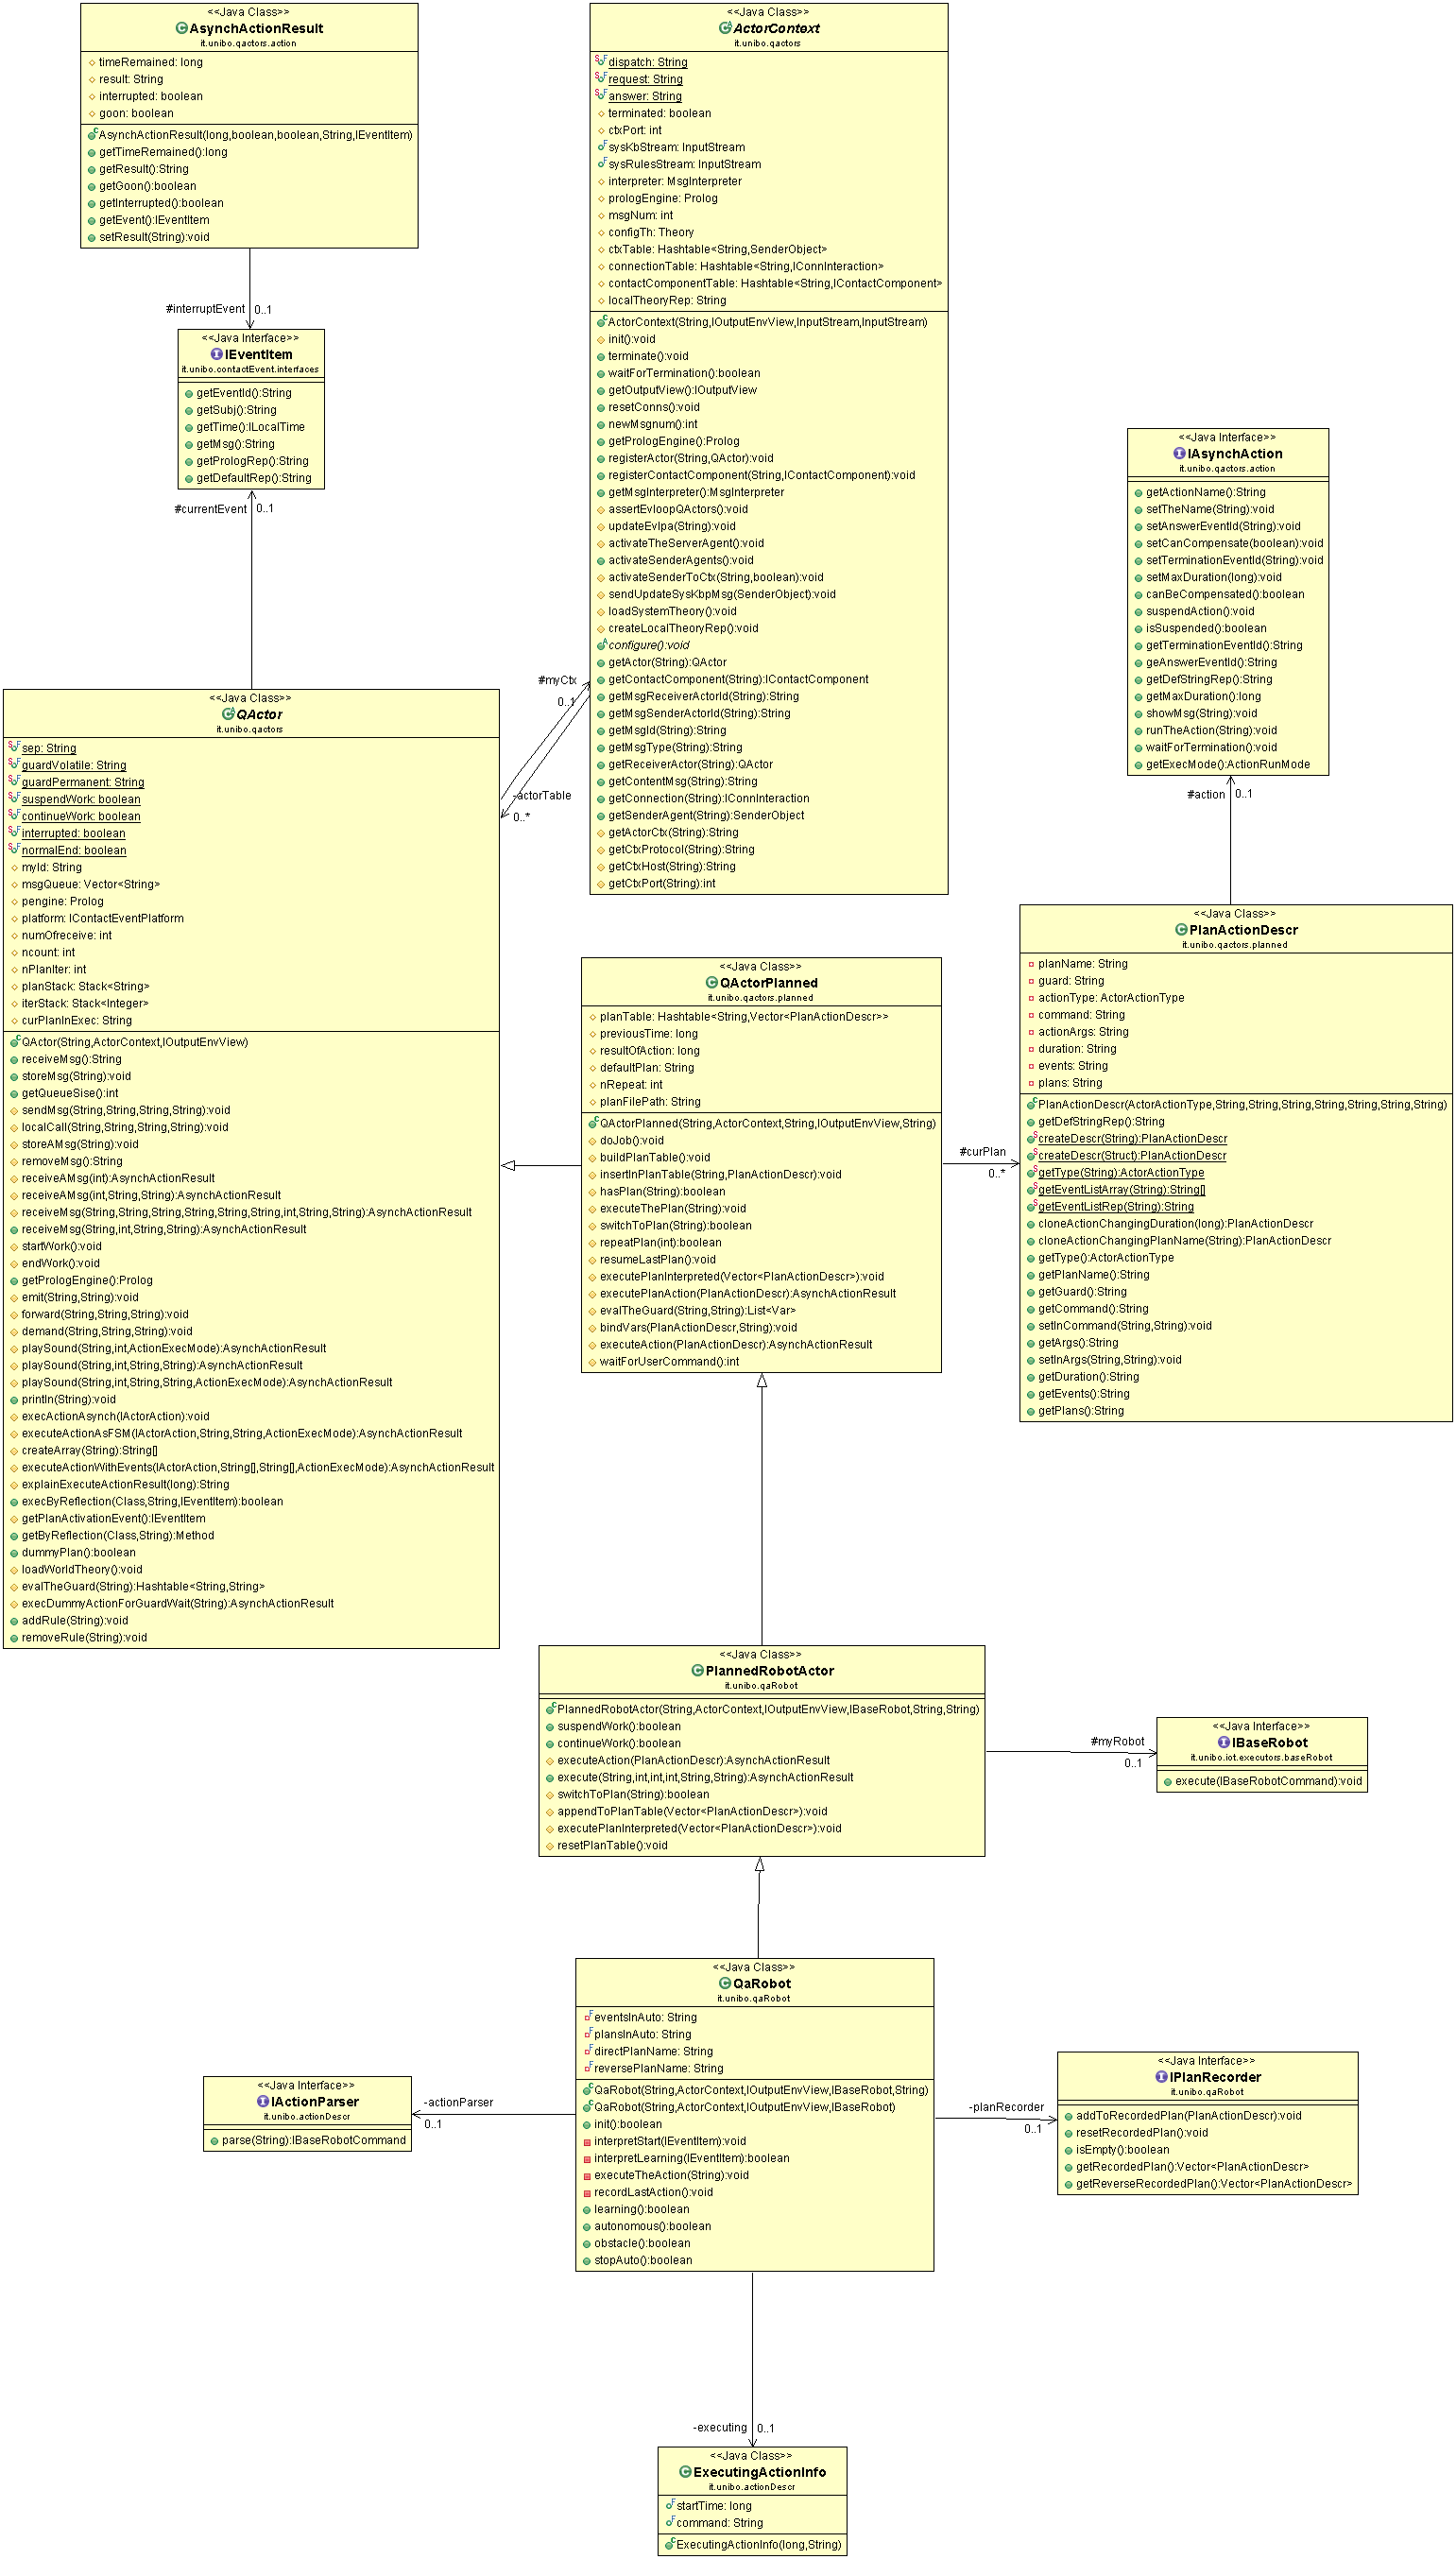
\includegraphics[width=12.5cm]{img/QaRobot.png}
\end{center}
QaRemote
\begin{center}
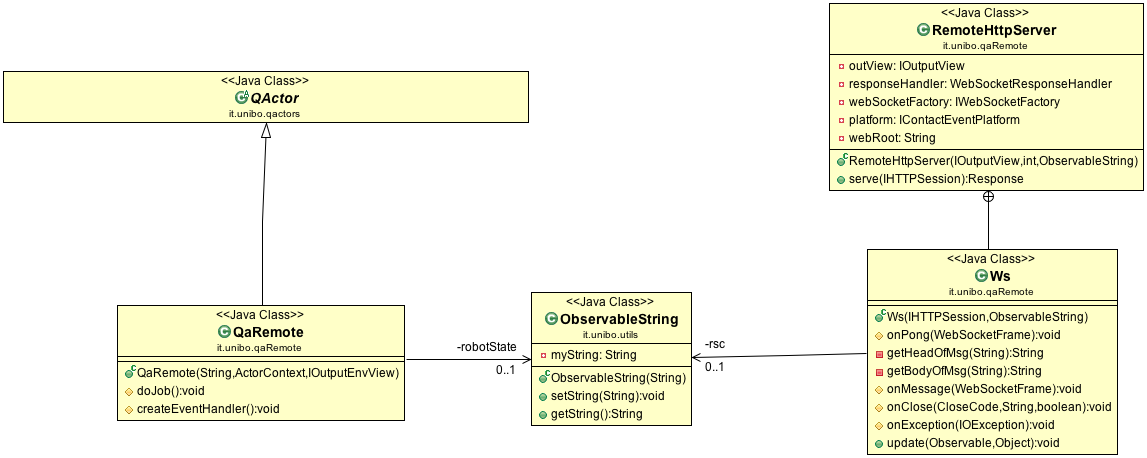
\includegraphics[width=12.5cm]{img/QaRemote.png}
\end{center}
%===========================================================================

\subsection{Structure}
According to the defined abstraction that led to our platform the model structure remains the same as the analysis one with the only difference that the communication is mediated by the contexts where the QActors are living in.
\subsection{Interaction}
\begin{center}
	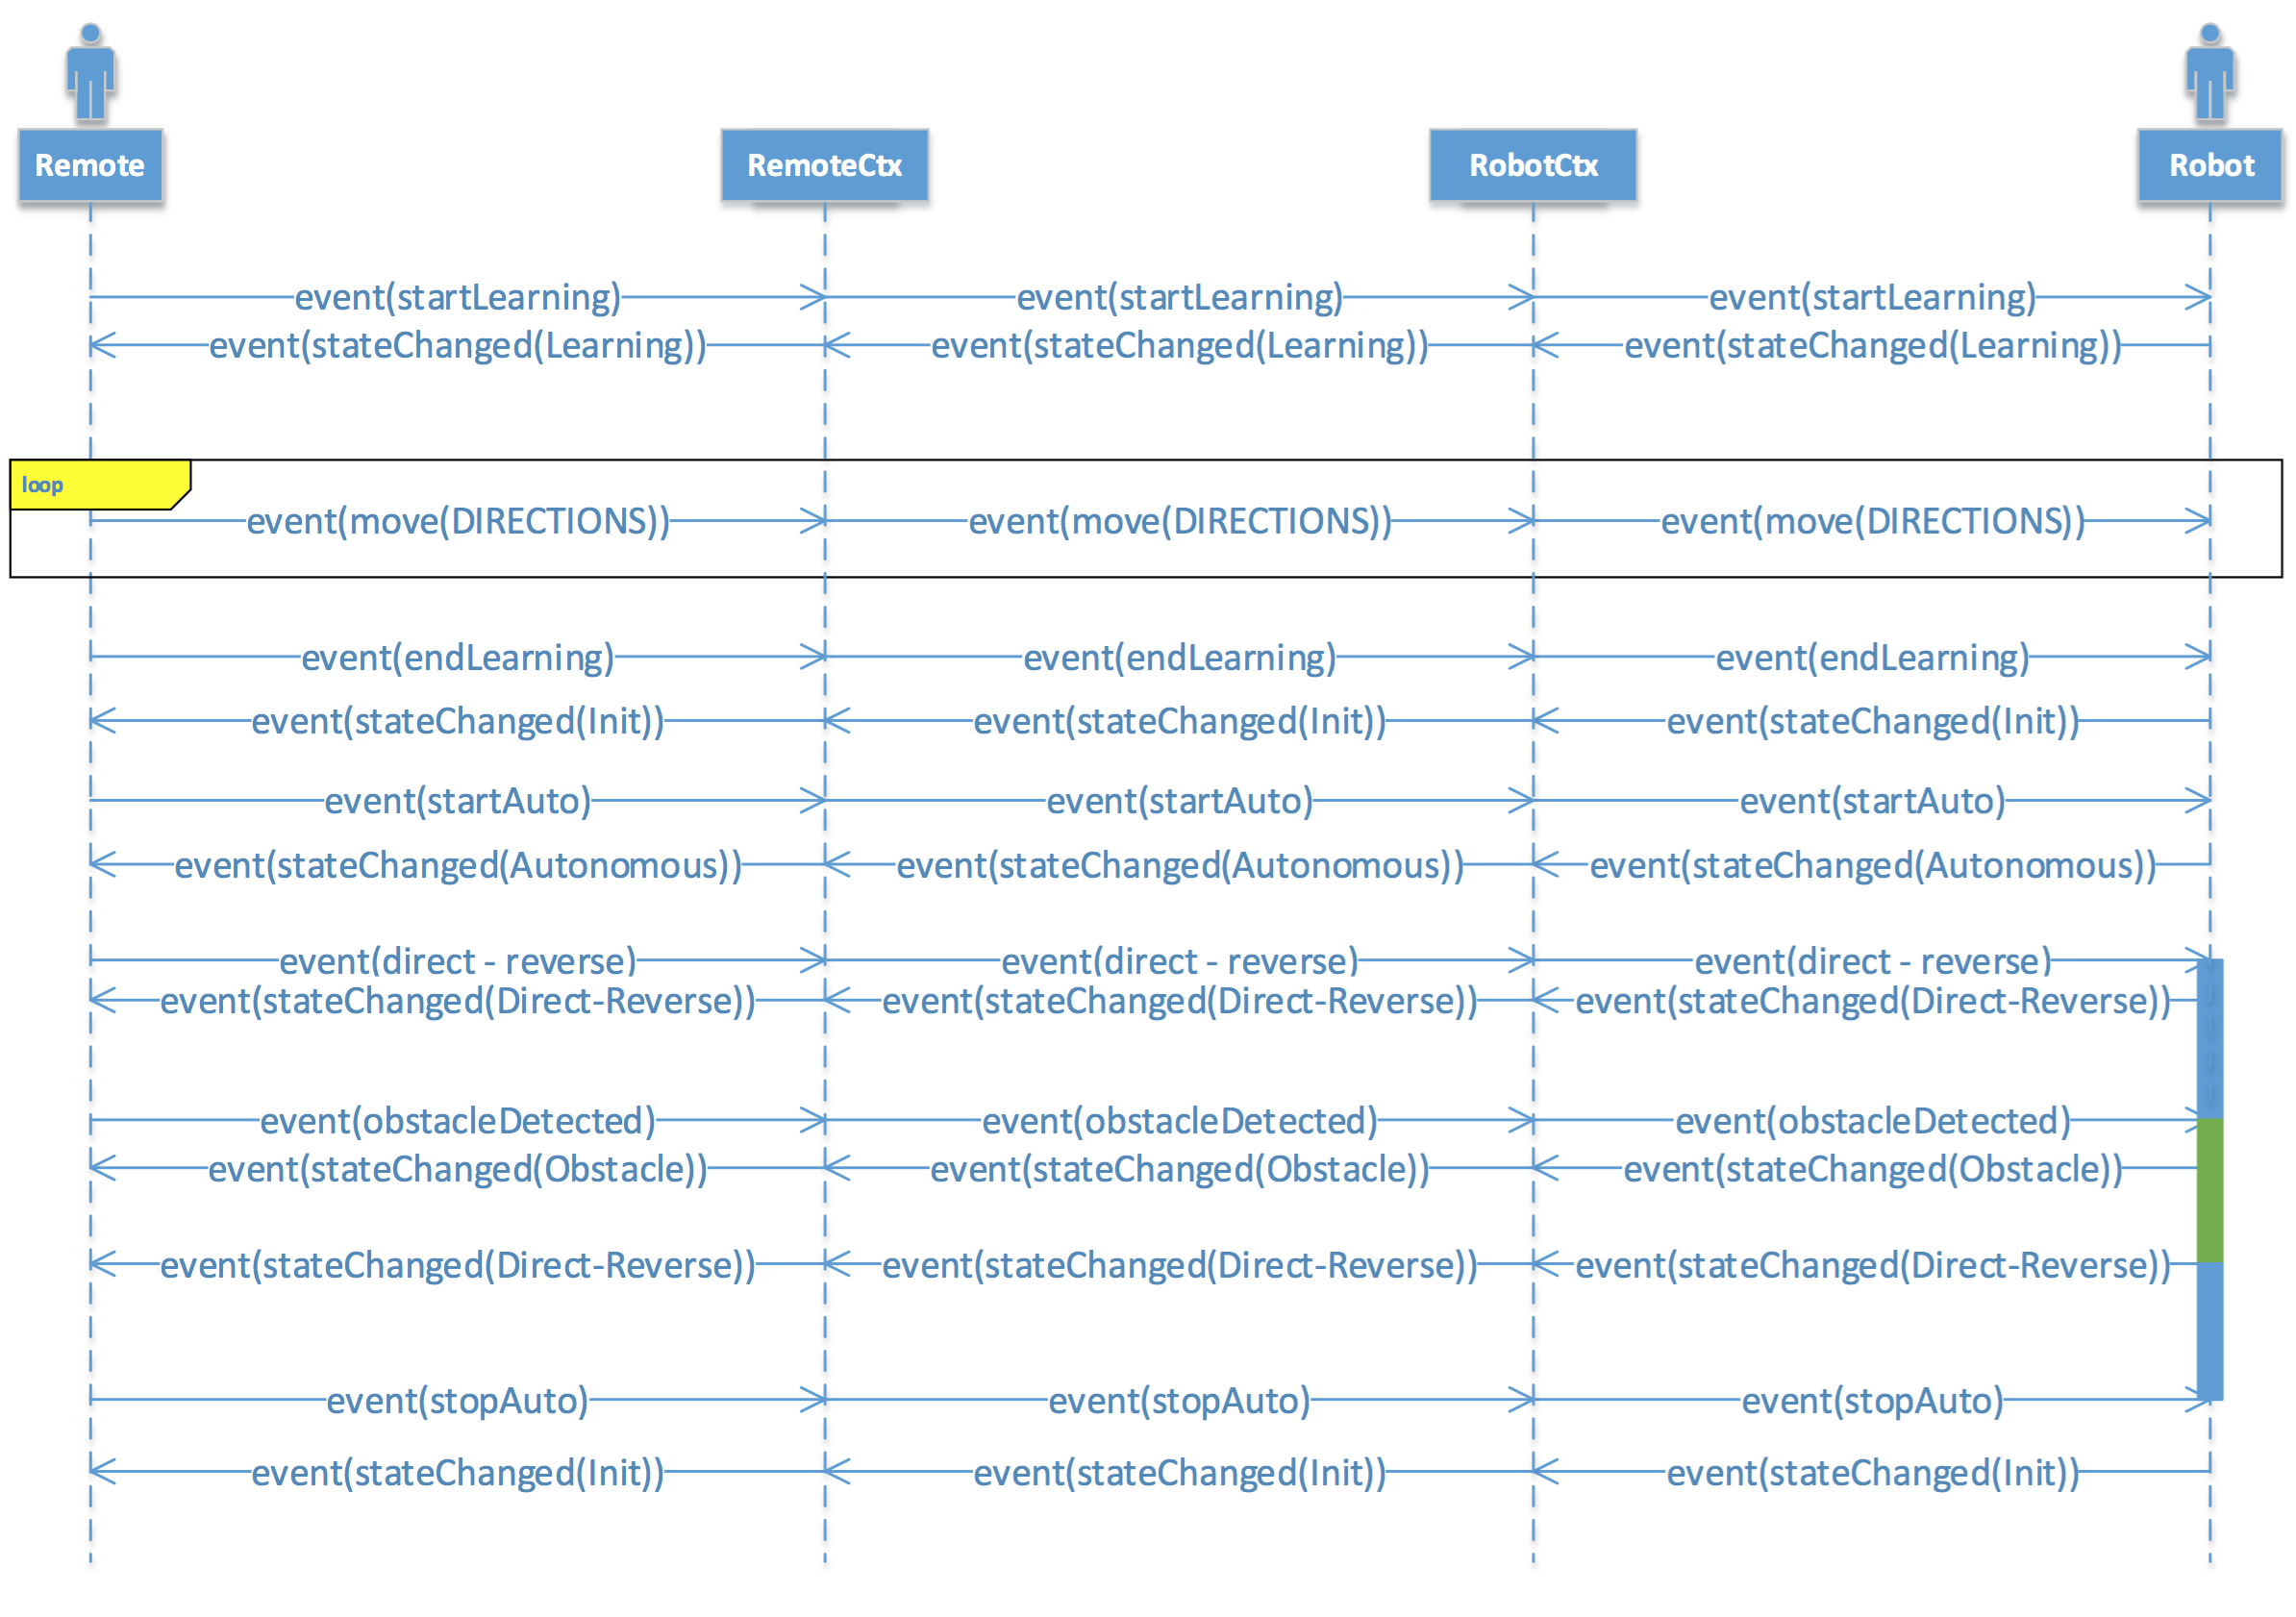
\includegraphics[width=13cm]{img/interaction_project.png}
\end{center}
\subsection{Behavior}
Taking advantage of the definitions of plans formalized during the abstraction gap chapter, we can realize a software artifact that is exactly the FSM formalized during the analysis step.\\
Regarding the Remote we realized that having a unresponsive remote (like the one of a Television) would be restrictive, so we realized a responsive GUI that enables only the commands permitted in that phase. To do that we modeled the Remote as a FSM that reacts to the state change of the robot.
%===========================================================================
\section{Implementation}
\labelsec{Implementation}
%===========================================================================

%===========================================================================
\section{Testing}
\labelsec{testing}
%===========================================================================

%===========================================================================
\section{Deployment}
\labelsec{Deployment}
To deploy the developed system we decided to use Raspberry Pi as main board for the robot equipped with Java and Pi4j library where we will load the developed code as Java Jar file.
For the remote controller we chose to develop the user interface as a web page that will be accessible in a uniform way from mobile devices and desktop ones.\\
The remote web page will be accessible through the Raspberry Pi network connections (Ethernet and Wi-Fi).
%===========================================================================

%===========================================================================
\section{Maintenance}
\labelsec{Maintenance}
Monotonic Extension
We will discuss how easy is to add functionalities to our software product.
We said that in our platform we can express the model through a formal language that leads to a code generation process. This way adding functionalities is simply a matter of explaining  them in our formal language. Infact we can describe all the entities in the system, their interactions and the data exchanged by those entities.
In order to explain this concept we will go through the process that let us add a new functionality to our robot:
-The new functionality is to let the Robot be reactive to Obstacle presence during the Autonomous Phase.

In order to do that we added a new event to our DSL file (from now on .qa  file), then we added a plan that handles the event. Then we explicated that actions during the Autonomous Phase are sensible to the obstacle event reacting with the defined obstacle handling plan.
%===========================================================================

%===========================================================================
\section{Discussion}
\paragraph{Requirement analysis}

\labelsec{Discussion}
%===========================================================================
discutere dell'evento nel caso sia generato dal nulla o da altro
dire come rappresentarlo visto che non possiamo farlo in uml
introduzione del sistema ad attori rispetto a java
problema se in analisi dei requisiti parlare dell'indipendenza dalla tecnologia
cambiamento dell'fsm del remote in fase successiva
%===========================================================================
\newpage
\appendix
\section{Codice}cl
\section{Information about the author}
\labelsec{Author}
%===========================================================================
\appendix
%===========================================================================
\vskip.5cm
%%% \begin{figure}
\begin{tabular}{ | c |  }
	\hline
	Photo of the Author\\
   	
\includegraphics[width=5cm]{img/zano.jpg}\\
	\hline
\end{tabular}
 
\appendix


\bibliographystyle{abbrv}
\bibliography{biblio}

\end{document}












